\documentclass{article}
\usepackage{tikz}
\usetikzlibrary{arrows}
\usepackage[english]{babel}
\usepackage[utf8]{inputenc}
\usepackage{minted}
\usepackage{fancyhdr}
\usepackage{graphicx}
\usepackage{amsmath}
\usepackage[margin=1in]{geometry}

\addtolength{\topmargin}{.2in}
\graphicspath{{.}}
 
\pagestyle{fancy}
\fancyhf{}
\rhead{Austin Bursey , Aaron Exley\\ Tim McGill, Joseph Myc}
\lhead{CP468 Term Project\\December 2nd  2019}
\rfoot{Page \thepage}
\begin{document}

\begin{titlepage}
  \pagestyle{fancy}
  \thispagestyle{fancy}
   \begin{center}
       \vspace*{1cm}
 
      \Huge
       \textbf{Term Project}
 
       \vspace{0.5cm}
       \Large
        CP468 \\ December 2nd 2019
 
       \vspace{1.5cm}
 
       \textbf{Austin Bursey , Aaron Exley, Tim McGill, Joseph Myc}
 
       \vfill

       \vspace{0.8cm}
 
   \end{center}
\end{titlepage}
\setcounter{page}{2}

\section{How to install/compile/execute our code}
To install the app simply download the .zip file and extract the files wherever you would like to keep them.
\\
Our code is written in python so no pre-compilation required. However, Python 3.6 or greater is required to run the code. \\
\\
We are using some external libraries that need to be installed.  To install these libraries use the following command. The libraries include numpy for faster and easier array calculations and matplotlib to plot graphs\\
\begin{center}
pip install -r requirements.txt
\end{center}
The code can be executed in multiple different ways from command prompt with different arguments:\\

--n [n] for specifying n-queens, 8 otherwise.\\
\\
--file [file] file as input for the initial board state, random otherwise.\\
\\
--maxsteps [steps] the amount queens to move until program should quit looking for a solution, 4000 otherwise. \\

Ex:
\\
To run random 8-queens examples: 
\begin{center}
python n-queens.py
\end{center}
To run random n-queens
\begin{center}
python n-queens.py --n 'n-value here'\\
or\\
python n-queens.py 'n-value'
\end{center}
To run a specific n-queens
\begin{center}
python n-queens.py --file 'file name here'
\end{center}
The format for the input file are as follows; a single digit per line representing the row for the queen. The queens are then filled in from descending order of the text file into the furthest left column of the board all the way to the furthest right in order. 

\section{Design and Implementation choices}
 We used structures like numpy arrays and dictionaries to improve performance. We also created two classes One called Queen which contains two variables; row and col for the row and column value respectively. And Puzzle which contains an array of type Queen which contains all the queens on the belonging to the current board state named 'queens' an array of type queens which contains all the queens currently attacking another queen and a count of all attacking pairs of queens.\\
 \newpage
 \subsection{Design} 
 1. When initializing a random board state we designed it in such a way that the next queen will be placed in one of the rows that will cause the least amount of conflicting queens (row will be chosen randomly among minimums if there's multiple).  \\
 \\
 2. After initialization, we count conflicting pairs of queens and store it in the Puzzle object as a variable. \\ 
 \\
\newline
 3. From there we check if the board is solved. If it is a solution, ie no conflicting queens exist, the board state is printed (for small N -values) and the user is informed a solution has been found. If the board state after generation is not a solution we call the local search algorithm.\\
 \\
 4. The local search algorithm takes in 3 parameters; the puzzle in its current state, the maximum number of steps you would like to the algorithm to run for. And the value of N of the current board size. From there the algorithm picks a conflicting queen from the array of conflicting queens and finds the possible positions to move that queen that will cause the minimum conflicts (if there is multiple minimums we pick randomly ). \\
 \\
 5. If a local minimum occurs we save the position of all the conflicting queens and force the program to find a minimum that does not involve moving a queen to a position it has already visited during this local minimum, which forces side-ways moves in a single direction.\\ 
  \\
 \subsection{Implementation}
 1. In order to maintain a linear run time, we had to be careful about how we went about counting the total amount of conflicts. The algorithm we went with was first to store the queens in an array of length N.
 Then in order to count the number of conflicts, we store 3 arrays one of size N that stores the number of queens in each row, and 2 of size 2N that store the number of queens in each of the 2 diagonals. We then loop
 through the N queens and increment each of the arrays by 1 as follows, $row[row\_of\_queen], backslashDiagonal[row + col], forwardslashDiagonal[N - row + col]$. Then to count the total amount of we loop through these arrays and for every element
 we add $(x(x - 1)) / 2$ conflicts to the total since every queen conflicts with each other which makes it a connected graph. We then use the same idea to find the minimum conflict spots when trying to move a queen.\\
 \\
 2. We also used numpy arrays and operations when ever we could as numpy is super optimized c code under the hood which would make the array operations we are doing not only easier to do, but also more efficient.
\\
\section{Performance for Different values of N}
Due to our design choices and implementation the board generation is the most computationally heavy part of the program, The graphs below shows how board generation and subsequently the entire program runs for different values of n. As you can see, the time increase for large values up to 100 000 is basically done in linear time, We begin to see quadratic run-time for any value of n larger than 100 000.\\
\\
\section{Graphs For n= 1 000 000}
The output of the program: \\
\\
python n-queens.py 1000000\\
Generating board\\
Progress: 999000/1000000\\
Board Generated in 5985.30265s\\
Initial Pairs = 6\\
BenchMark: 0\\
Time: 230.99690s\\
=====================SOLUTION FOUND IN 40 STEPS=====================  \\     
Pairs = 0\\
\\
The graph for the number of conflicting queens per move: 
\begin{center}
  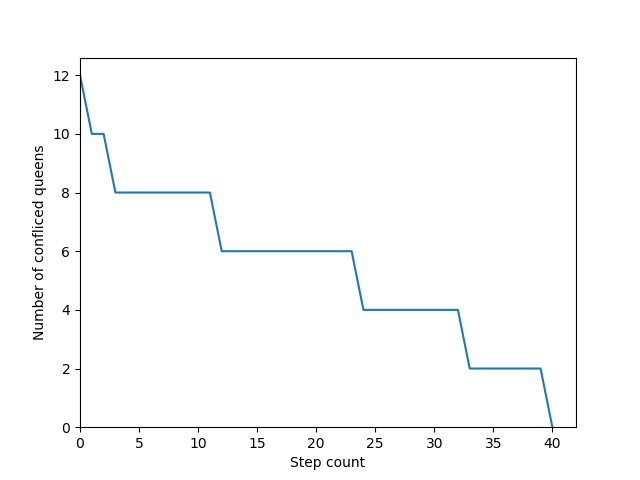
\includegraphics[scale=0.6]{n-queens-conflict-count-plot-1000000}
\end{center}
The graph for the number of pairs of conflicting queens per move: 
\begin{center}
  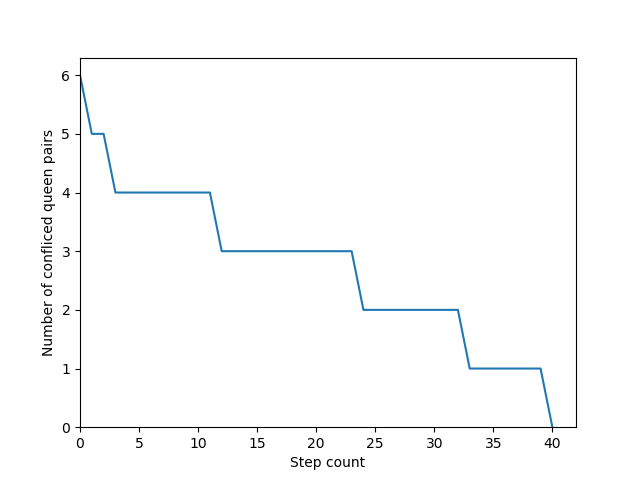
\includegraphics[scale=0.6]{n-queens-conflict-pair-count-plot-1000000}
\end{center}

\section{Results for test runs on different n-values}
Run Times 
\begin{center}
  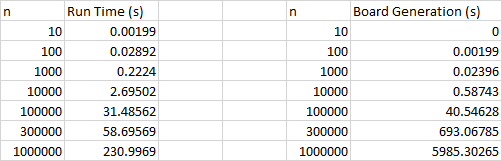
\includegraphics[scale=0.6]{RunTimesChart}
\end{center}
Board Generation run-time graph:
\begin{center}
  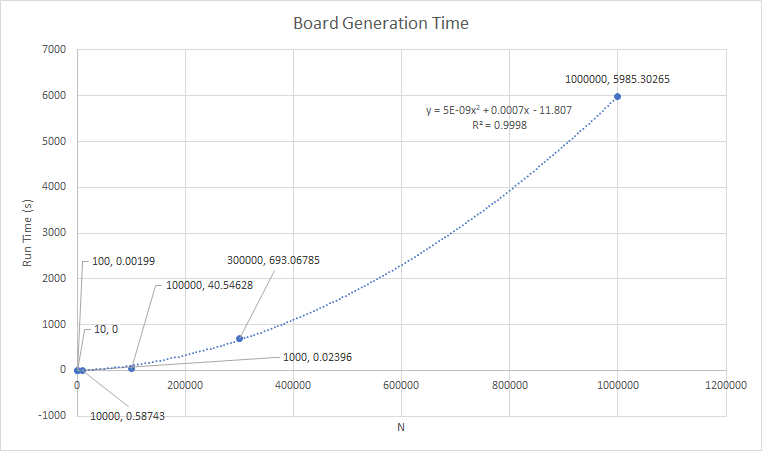
\includegraphics[scale=0.6]{boardGenerationTimePlot}
\end{center}
\newpage
Local Search run-time graph 
\begin{center}
  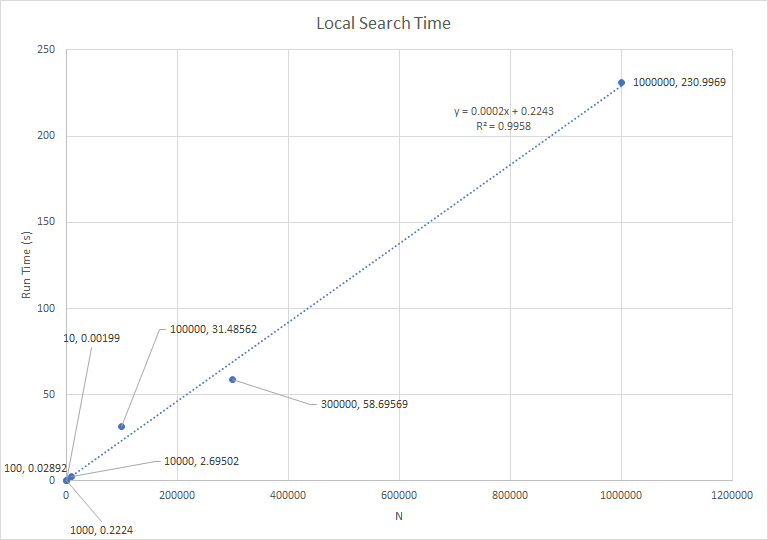
\includegraphics[scale=0.6]{localSearchTimePlot}
\end{center}

\section{Poster of Large n-queen Solution}
Provided in the zip file with the code, the file name is 1000-queen-poster.png
\section{Code}
\begin{minted}{python}
  from random import randint
  from operator import add
  import time
  import sys
  import argparse
  from PIL import Image
  from PIL import ImageDraw
  from PIL import ImageFont
  
  import numpy as np  # pip install numpy
  import matplotlib.pyplot as plt # pip install matplotlib
  
  class Queen: 
      def __init__(self, col ,row, pairs=0): 
          self.col = col 
          self.row = row
          self.pairsCount = pairs
    \end{minted}
\newpage
\begin{minted}{python}    
      def __str__(self):
          return '\nCol={}, Row={}'.format(self.col, self.row)

      def __repr__(self):
          return '\nCol={}, Row={}'.format(self.col, self.row)

      def __eq__(self,other): 
          return self.col == other.col
  
      def __ne__(self,other):
          return not self.__eq__(other)
  
  class puzzle: 
      def __init__(self, n, array=None): 
      
          self.queens = []
  
          #If parameters for the positions of the queens are passed in, 
          #add these positions to the puzzle        
          if array is not None:
              n = len(array)
              for i in range(n): 
                  self.queens.append(Queen(i, array[i]))
  
          #If parameters for the queens positions are not passed in, create a random minimized board.
          else : 
              self.queens = createBoard(n)
  
          self.conflictQueens = []
          self.pairsCount = countPairs(self, n)
          
      def __str__(self):
          return '\n Pairs = {}\n conflicted Queens = {}'.format(self.pairsCount, self.conflictQueens)
  
      def __repr__(self):
          return '\n Pairs = {} conflicted Queens = {}'.format(self.pairsCount, self.conflictQueens)
    
  def createBoard(N):
      '''
      Creates the inital state of the board by adding the next queen to the spot 
      with the least conflicts O(2n^2)
      ---------------------------
      Params:
          n: the size of the board
      returns:
          puzzle: a 1-d list of size n containing a queen at each column
      '''
  
      #Queen location in the row
      row = np.zeros(N, dtype=np.int16)
  
      #Top left to bottom right diagonal array
      ld = np.zeros(N + N, dtype=np.int16)
  \end{minted}
\newpage
\begin{minted}{python}   
      #Top right to bootm left diagonal array
      rd = np.zeros(N + N, dtype=np.int16)

      r = np.random.randint(0, N)
   
      #Add initial queens constraints to the board
      row[r] = 1
      ld[r] = 1
      rd[N - r] = 1
  
      #Add initial queen to the board
      queens = [Queen(0, r)]
  
      for col in range(1, N): # O(N)
  
          #Print progress check every so often
          if N >= 100000:
              if col % 1000 == 0:
                  print("Progress: {}/{}".format(col, N), end='\r') 
  
          #Get diagonal array of collision counts
          p = ld[col: col + N]
          q = (rd[col + 1: col + N + 1])[::-1]
          #Get array of all collision counts
          total = row + p + q # O(N)
  
          #Get positions with the minimum number of collisions
          minT = np.where(total == total.min())[0] # O(N)
  
          #Pick random location with minimum number of collisions
          r = np.random.randint(0, minT.shape[0])
          r = minT[r]
  
          #Add constraints to the board
          row[r] += 1
          ld[r + col] += 1
          rd[N - r + col] += 1
  
          #Add queen to the board
          queens.append(Queen(col, r))
      print()
      return queens
  
  def countPairs(puzzle, n):
      '''
      Counts the total number of pairs in the board O(4n)
      ---------------------------
      Params:
          puzzle: A puzzle for the current state
          n: the size of the board
      returns:
          counts: the count of the pairs
      '''
      count = 0
      f_row = [0] * n
      f_mdiag = [0] * (n + n)
      f_sdiag = [0] * (n + n)
      queens = puzzle.queens
      puzzle.conflictQueens = []
  
      cRow = dict({})
      cmD = dict({})
      csD = dict({})
  
      #Count how many queens are in each row, and diagonal
      for i in range(n): # O(n)
  
          row = queens[i].row
  
          f_row[row] += 1
          if f_row[row] > 1:
              cRow[row] = True
  
          f_mdiag[row + i] += 1
          if f_mdiag[row + i] > 1:
              cmD[row + i] = True
  
          f_sdiag[n - row + i] += 1
          if f_sdiag[n - row + i] > 1:
              csD[n - row + i] = True
  
      #Count total number of pairs
      for i in range(n + n): # O(2n)
          x, y, z = 0, 0, 0
  
          if i < n:
              x = f_row[i]
          y = f_mdiag[i]
          z = f_sdiag[i]  
          count += (x * (x - 1)) // 2
          count += (y * (y - 1)) // 2
          count += (z * (z - 1)) // 2
  
      #Count the number of queen conflicts in the puzzle object and add it to
      # the puzzle's array conflictQueens
      for q in queens: # O(n)
          if q.row in cRow or q.row + q.col in cmD or n - q.row + q.col in csD:
              puzzle.conflictQueens.append(q)
  
      return count
   \end{minted}
\newpage
\begin{minted}{python}
  def localSearch(puzzle, maxSteps, n):
      '''
      Performs min conflics local search of the puzzle O(6n)
      ---------------------------
      Params:
          puzzle: A puzzle for the current state
          maxSteps: The maximum number of steps to try before aborting
          n: the size of the board
      returns:
          The finished puzzle
          The number of steps
          If it was solved
      '''
      global conflicts
      global conflictspair
      savedInstances = dict({})
      blacklistedQueens = []
      lastCount = 0 
      thisCount = 1
      for i in range(maxSteps): # O(k)
          if i % 100 == 0: 
              print("Amount of Steps: {:5}".format(i), end='\r')
  
          #If a local minimum is hit, mark all queens that have colissions for moving/adjusting.
          if lastCount == thisCount:
              for queen in puzzle.conflictQueens: 
                  if (queen.col, queen.row) not in savedInstances: 
                      savedInstances[(queen.col,queen.row)] = True
          else : 
              savedInstances = dict({})
  
          m = len(puzzle.conflictQueens)    
  
          index = randint(0, m - 1)
          currentQueen = puzzle.conflictQueens[index]
  
          #Get new location to move the queen to O(2n)
          pairMin, minRow = findMinimum(currentQueen.row,currentQueen.col, puzzle,n,savedInstances)
               
          #If the row to adjust is not the current row, move to the row and save the new instance
          if (minRow != currentQueen.row): 
              puzzle.queens[currentQueen.col].row = minRow
              puzzle.queens[currentQueen.col].pairsCount = pairMin
              if (currentQueen.col, currentQueen.row) not in savedInstances: 
                  savedInstances[(currentQueen.col,currentQueen.row)] = True
          #Otherwise, just save the instance
      
          puzzle.pairsCount = countPairs(puzzle,n) # O(4n)
          lastCount = thisCount 
          thisCount = puzzle.pairsCount
          #append count to conflict(s) array
          conflicts.append(len(puzzle.conflictQueens))
          conflictspair.append(puzzle.pairsCount)
          if puzzle.pairsCount == 0: 
              print()
              return puzzle, i, True
      print()
      return puzzle, i, False
       
  def findMinimum(cRow, cCol, puzzle, n, savedInstances):
      '''
      Finds the next move to do for a given queen that will minimize the conflicts O(2n)
      ---------------------------
      Params:
          row: The row of the current queen
          col: The column of the current queen
          puzzle: A puzzle for the current state
          n: the size of the board
          savedInstance: A small buffer of previous moves used for dealing with plateaus
      returns:
          The new count for the conflicts
          The row to move the queen too
      '''
  
      total = np.zeros(n)
      queens = puzzle.queens
  
      for i in range(n): # O(n)
  
          #count the collisions in each row except for the current row
          row = queens[i].row
          if i != cCol:
              total[row] += 1
  
          #Count collisions in the diagonals that pass through the current column
          if cCol <= row + i <= cCol + (n - 1):
              total[row + i - cCol] += 1
          if cCol + 1 <= n - row + i <= n + cCol:
              total[abs((n - row + i) - (n + cCol))] += 1
  
      mins = np.where(total == total.min())[0] # O(n)

      i = np.random.randint(0, mins.shape[0])
      r = mins[i]
  
      #Check that the move has not already been made
      while len(mins) > 1 and (cCol, r) in savedInstances:
          mins = np.delete(mins, i)
          i = randint(0, len(mins) - 1)
          r = mins[i]
      
      if len(mins) == 1:
          return total[mins[0]], mins[0]
      else:
          return total[mins[i]], mins[i]
  
   \end{minted}
\newpage
\begin{minted}{python}
  def saveBoardToImage(puzzle, n):
  
    img = Image.new('RGB', (6500, 7400), (255, 255, 255))
    d = ImageDraw.Draw(img)
    
    font = ImageFont.truetype("Courier Prime Code.ttf", 200)
    d.text((6500 // 2 - 500, 20), "1000-Queens", fill=(0, 0, 0), font=font)

    arr = puzzle.queens
    for i in range(n-1, -1, -1):#rows 
        board = ""
        for j in range(n):#column
            if arr[j].row == i:
                board += "Q"
            else:
                board += "."
        d.text((250, (n - i - 1) * 7 + 300), board, fill=(0, 0, 0))

    img.save("large.png")
  
  def printBoard(puzzle):
      '''
      Prints the board with index 0, 0 at the botton left corner
      ---------------------------
      Params:
          puzzle: A puzzle for the current state
      prints:
          prints the board
      '''
      arr = puzzle.queens
      for i in range(n-1, -1, -1):#rows 
          for j in range(n):#column
              if arr[j].row == i: 
                  print("Q|",end = "")
              else : 
                  print(".|",end="")
          print()
      print("Pairs = {}".format(puzzle.pairsCount))
  
  conflicts=[]
  conflictspair=[]
  if __name__ == "__main__": 
  
      parser = argparse.ArgumentParser(description="Solve n-queens")
  
      parser.add_argument("--n", default=-1, type=int, help="The size of the board (nxn) with n queens (default: 8)")
      parser.add_argument("--file", default=None, help="Read initial state of the board from a file")
      parser.add_argument("--maxsteps", default=4000, type=int, help="The maximum amout of steps to try before giving up")
      parser.add_argument('args', nargs='*', help="if an integer is put here it will be used as n if n is not provided")
  
      args = parser.parse_args()
   \end{minted}
\newpage
\begin{minted}{python}
      if args.n != -1:
          n = args.n
      elif len(args.args) > 0:
          n = int(args.args[0])
      else:
          n = 8
  
      if args.file is not None:
          initialPos = []
          with open(args.file, 'r') as f:
              for line in f:
                  initialPos.append(int(line))
          n = len(initialPos)
          newPuzzle = puzzle(n, initialPos)
      else:
          print("Generating board")
          t = time.time()
          newPuzzle = puzzle(n)
          print("Board Generated in {:.5f}s".format(time.time() - t))
  
      if n < 17:
          printBoard(newPuzzle)
      else:
          print("Initial Pairs = {}".format(newPuzzle.pairsCount))
  
      if newPuzzle.pairsCount != 0:
  
          t = time.time()
          solution, i, solved = localSearch(newPuzzle, args.maxsteps, n)
          print("Time: {:.5f}s".format(time.time() - t))
          if solved: 
              print("=====================SOLUTION FOUND IN {} STEPS=====================".format(i))
              if n < 17:
                  printBoard(solution)
              else:
                  print("Pairs = {}".format(newPuzzle.pairsCount))

              if n <= 1000:
                  saveBoardToImage(solution, n)
              # else : 
                  # print(solution)
          else: 
              print("=====================NO SOLUTION FOUND AFTER {} STEPS=====================".format(i))
              if n < 17:
                  printBoard(solution)
              else:
                  print("Pairs = {}".format(newPuzzle.pairsCount))
  
      #ploting the conflict count
      plt.plot(conflicts)
      plt.xlim(left=0)        
      plt.ylim(bottom=0)
      plt.ylabel('Number of confliced queens')
      plt.xlabel('Step count')
      plt.savefig('n-queens-conflict-count-plot.png')
      plt.close()
      #ploting the conflict pair count
      plt.plot(conflictspair)
      plt.xlim(left=0)        
      plt.ylim(bottom=0)
      plt.ylabel('Number of confliced queen pairs')
      plt.xlabel('Step count')
      plt.savefig('n-queens-conflict-pair-count-plot.png')
      plt.close()
\end{minted}

\end{document}